\section{About}\label{sec:about}

\begin{wrapfigure}{R}{0.3\textwidth}
\centering
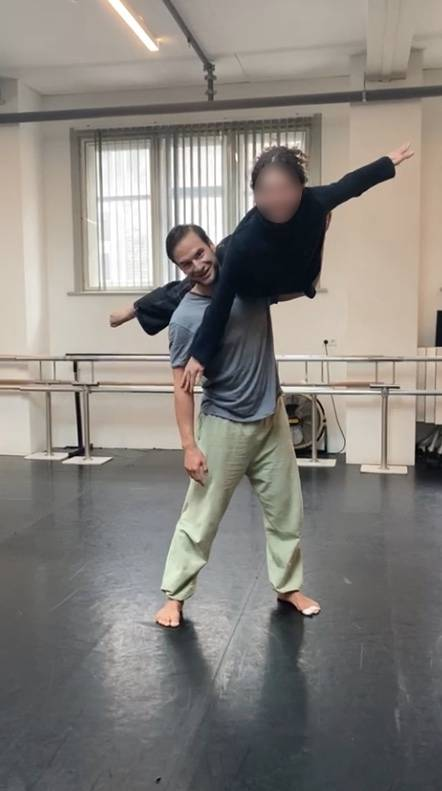
\includegraphics[width=0.25\textwidth]{images/about}
\end{wrapfigure}

What can you expect from this book, and who has written it?
Who is the target audience, and where lies the emphasis?
And some general remarks as a form of a disclaimer.

\subsection{Book}\label{subsec:book}

The following pages were initially written for the sole purpose of taking personal notes, but then it started to grow further and further, and now it serves its use to also others, whether beginners or more experienced alike, who are interested in getting more acquainted with the theoretical background of the fine art of Contact Improvisation Dance, or simply \textbf{CI} for short as of now (sometimes also called ``\textit{contact}'' or ``\textit{contact dance}'' in the community).

Whatever is written here does not claim to hold any absolute, objective truth, but merely is a manifestation of my very own personal, subjective collection of experiences, thoughts and opinions I gained over the last year within my very limited environment.
I also summarized all the information I stumbled upon along my path of exploration, might it be oral teachings, direct or indirect, or written information found in books or on the internet.
Whatever is written here is of course also partly biased, although I tried to do my best to free myself from my own limitations of my perception of reality as much as I could, and thus, sometimes the content will be colored by my personal (movement) background.

The book uses the masculine version in case both can be applied for the sake of simplicity and always implying of course that the female version could have been equally used as well.

\subsection{Myself}\label{subsec:myself}

My background is mainly Asian Internal Martial Arts, and as such, my focus lies more on a practical approach, where ``form follows function'', and less about any aesthetic aspects as some might consider to be an essential part of dancing in a more narrow definition.
Furthermore, as a body worker, I emphasize the importance of the non-verbal communication aspect of movement and touch, the softness and gentleness in listening skills and expression our own personality through this dance.

For me personally, the looks are not so important, and ``right'' is what is pragmatic, meaning efficient in time and space (thinking of anatomy, physics, and biomechanics), and as well whatever is in alignment with the principles of CI.
Besides those more physical aspects, the psychological aspect should be granted at least half of the attention: The benefit for one's mental health, the ability to get to know oneself and others more deeply, and of course a more philosophical/spiritual path which can also be walked with the help of this deep art.
